\section{Resultados y conclusiones principales}


De la metodología anterior, se obtienen los siguientes resultados.\\

\begin{figure}
    \centering
    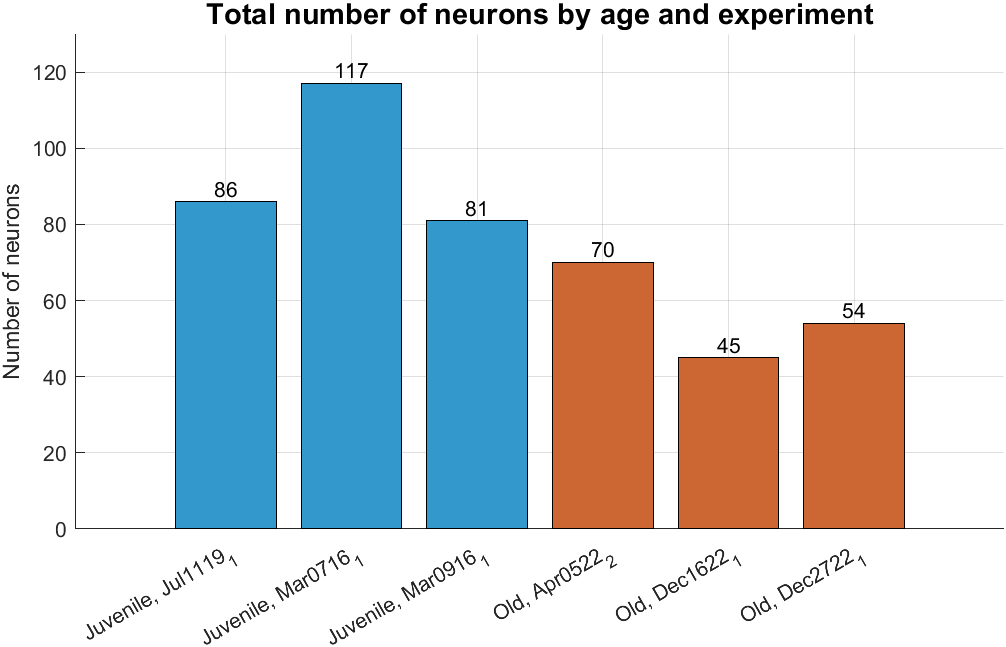
\includegraphics[width=0.6\textwidth]{img/Total_Neurons.png}
    \caption{Total de neuronas por set de datos.}
    \label{total_neurons}
\end{figure}

\begin{figure}
    \centering
    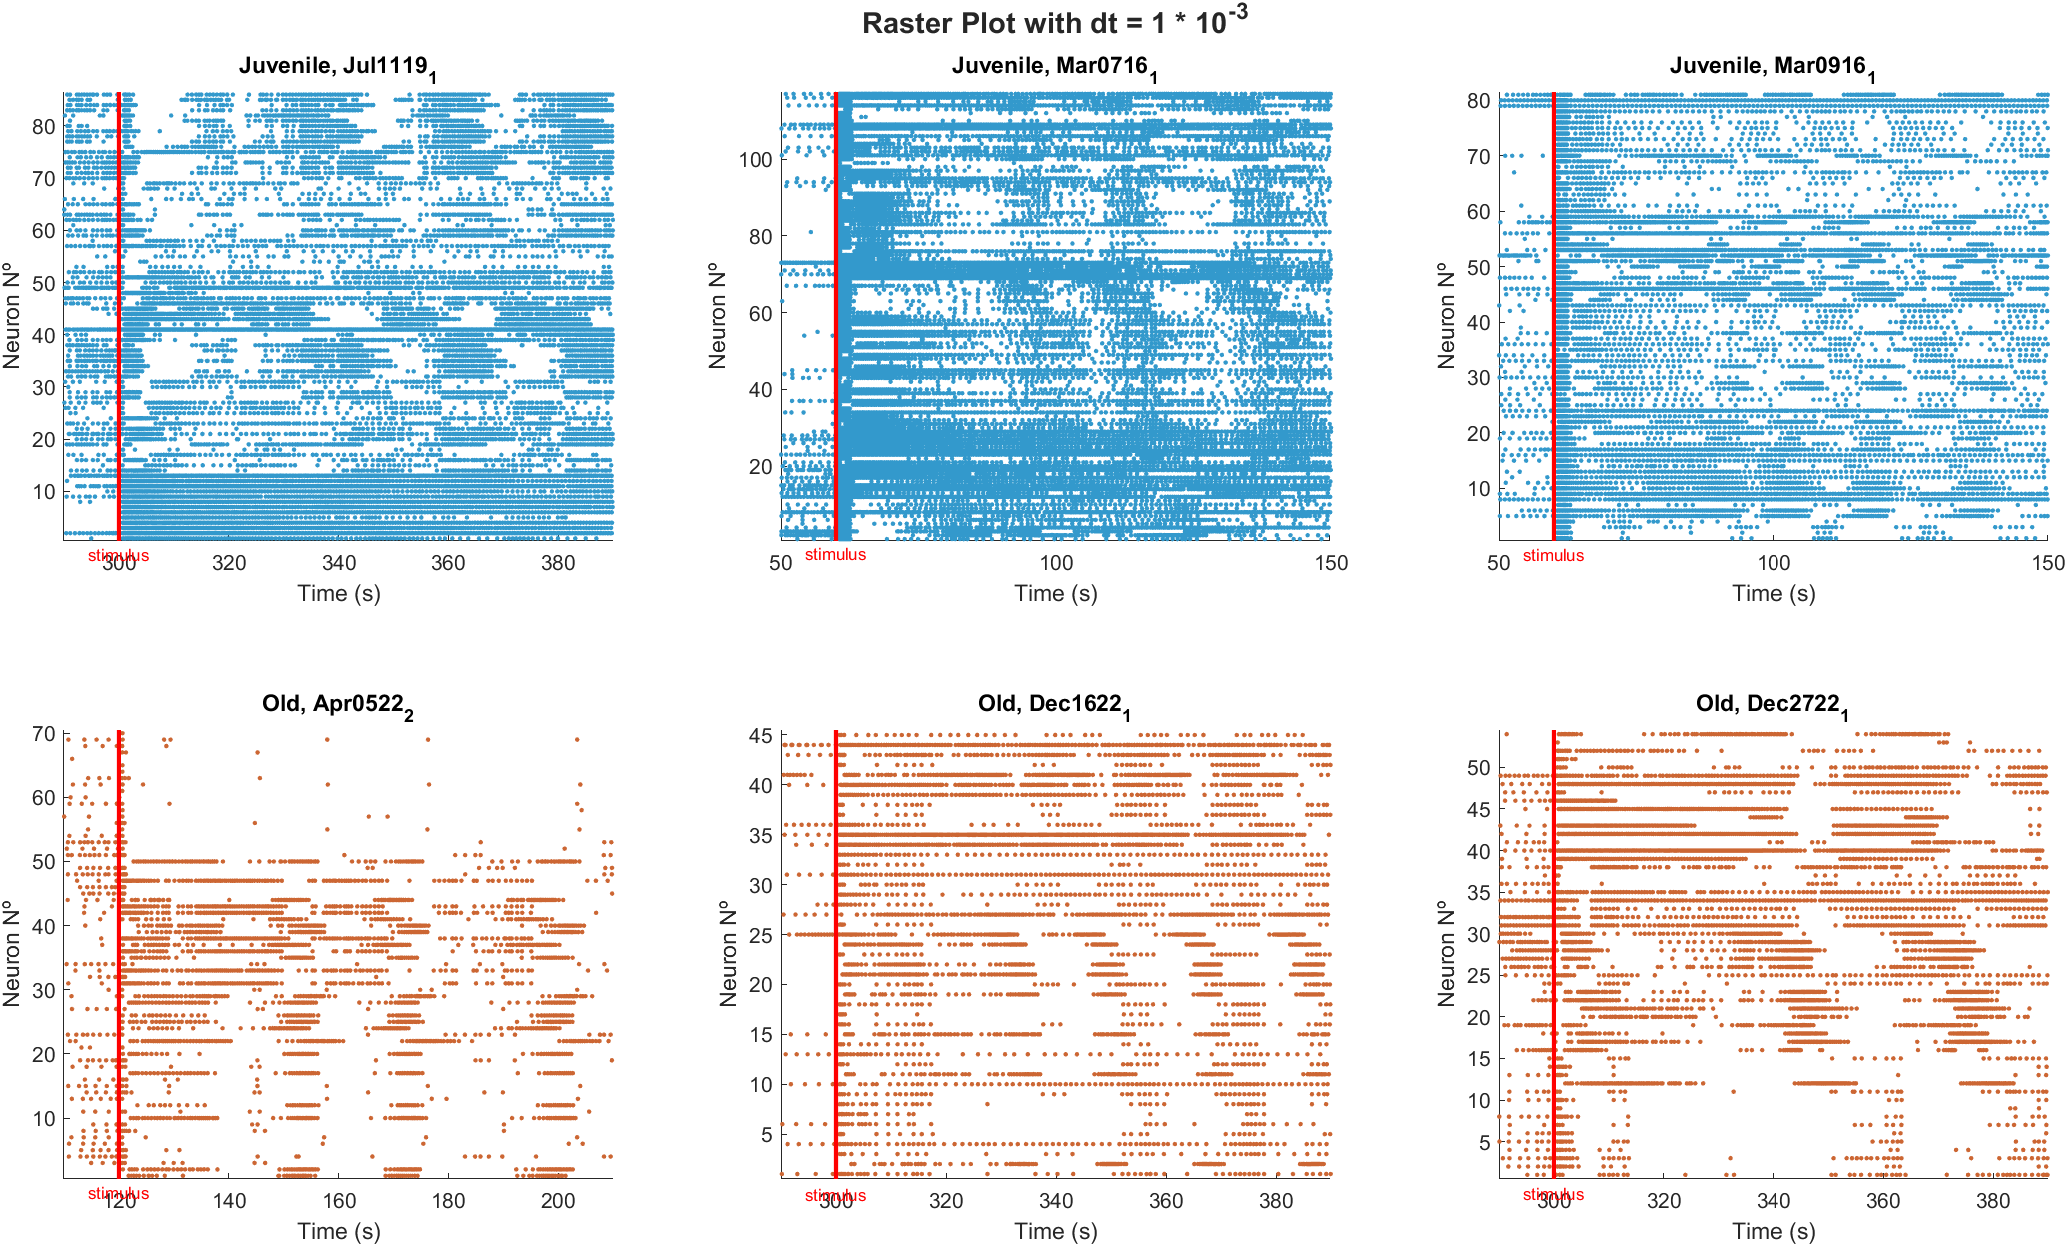
\includegraphics[width=0.9\textwidth]{img/RasterPlot.png}
    \caption{Raster Plot por set de datos.}    
    \label{rasterplot}
\end{figure}

\begin{figure}
    \centering
    \subfloat{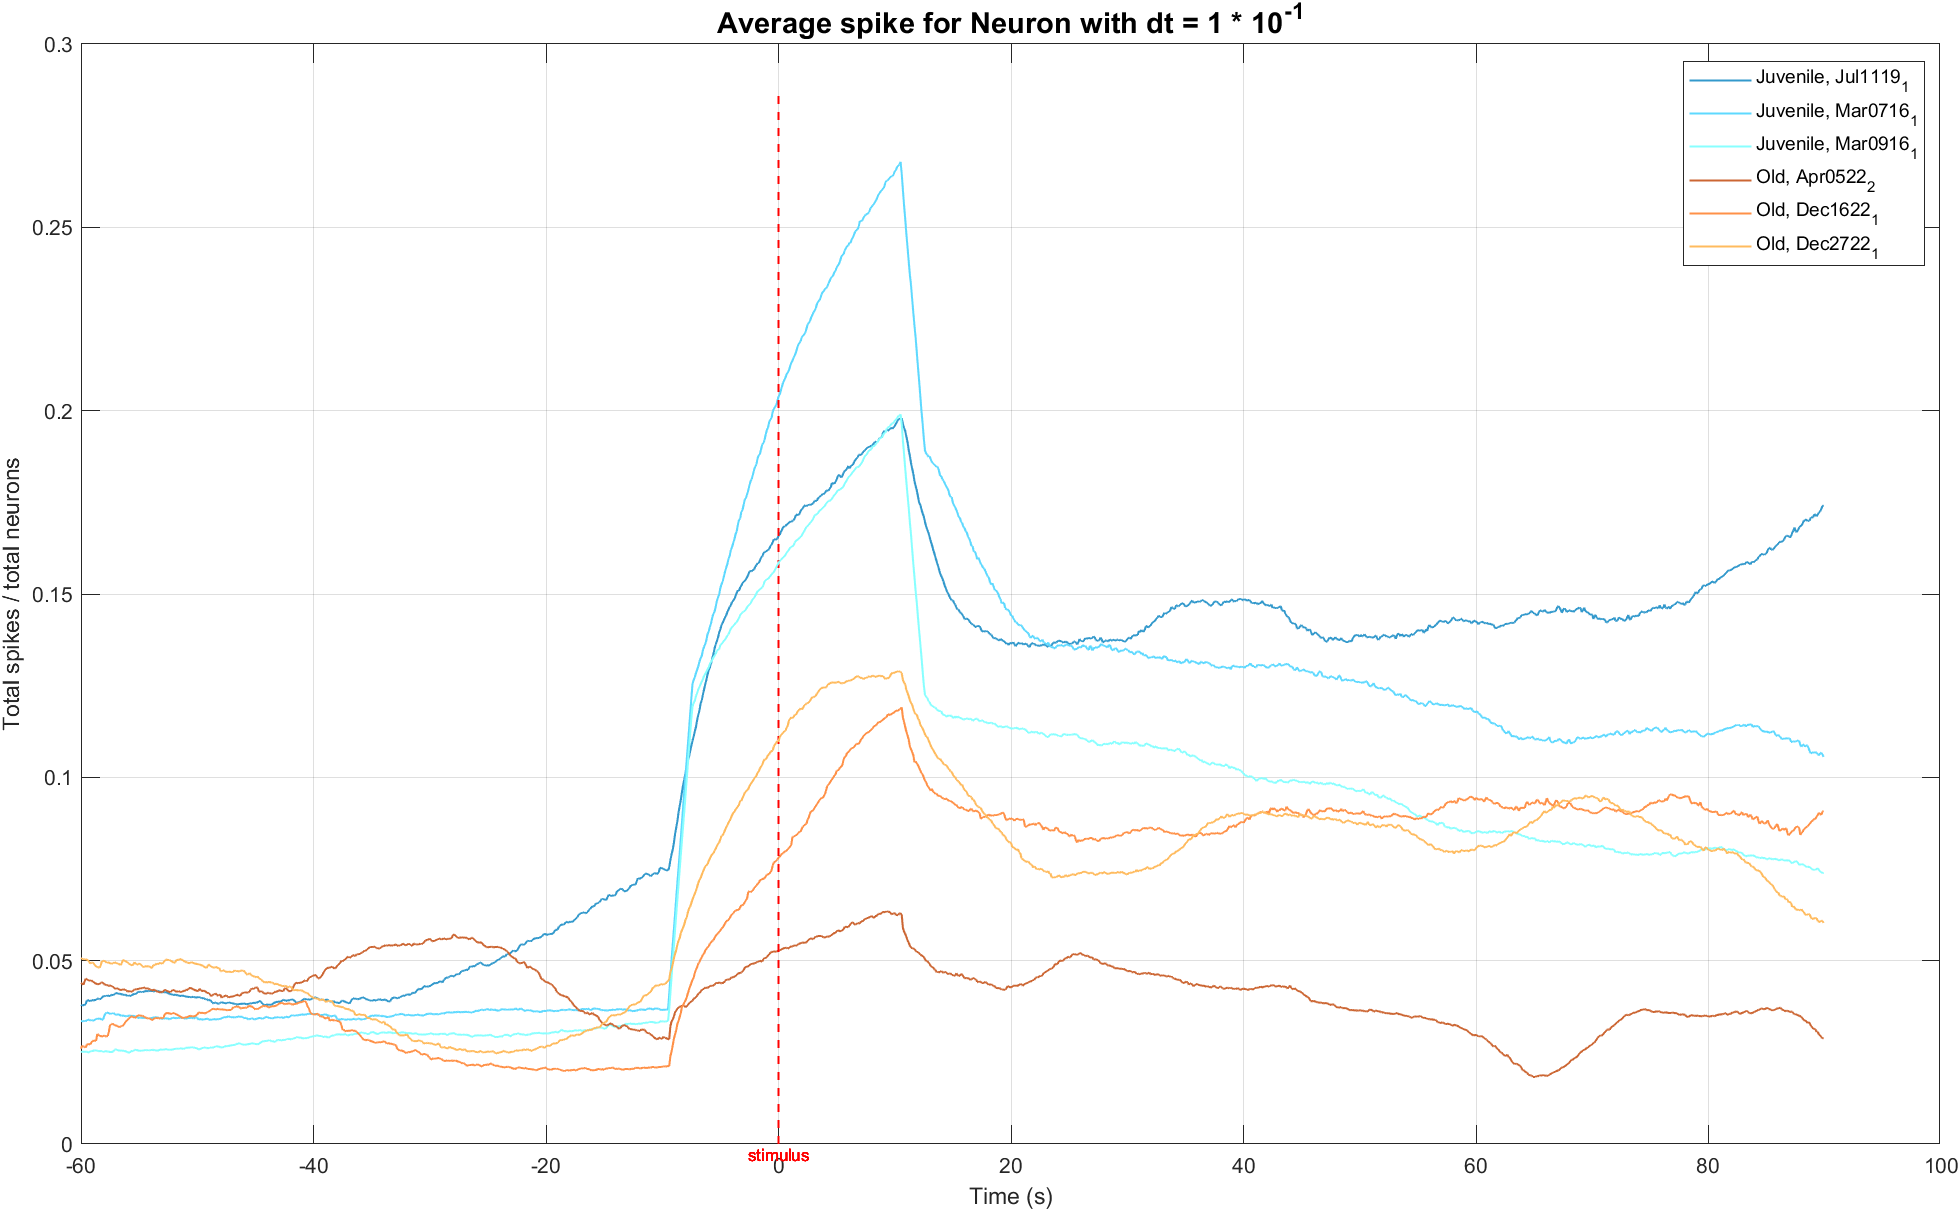
\includegraphics[width=0.8\textwidth]{img/Average_spike_for_Neuron.png}}
    
    \hfill
    
    \subfloat{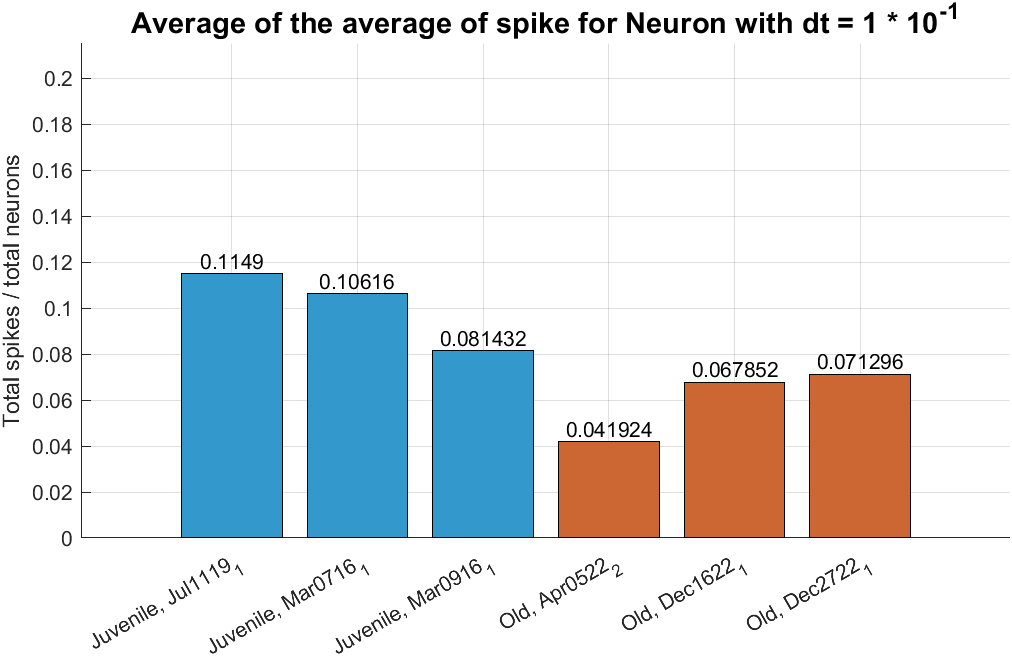
\includegraphics[width=0.7\textwidth]{img/Average_of_the_average_spike_for_Neuron.png}}
    
    \caption{Promedio de spikes totales normalizado por cantidad total de neuronas por set de datos.}
    
    \label{promdelprom}
\end{figure}

\begin{figure}
    \centering
    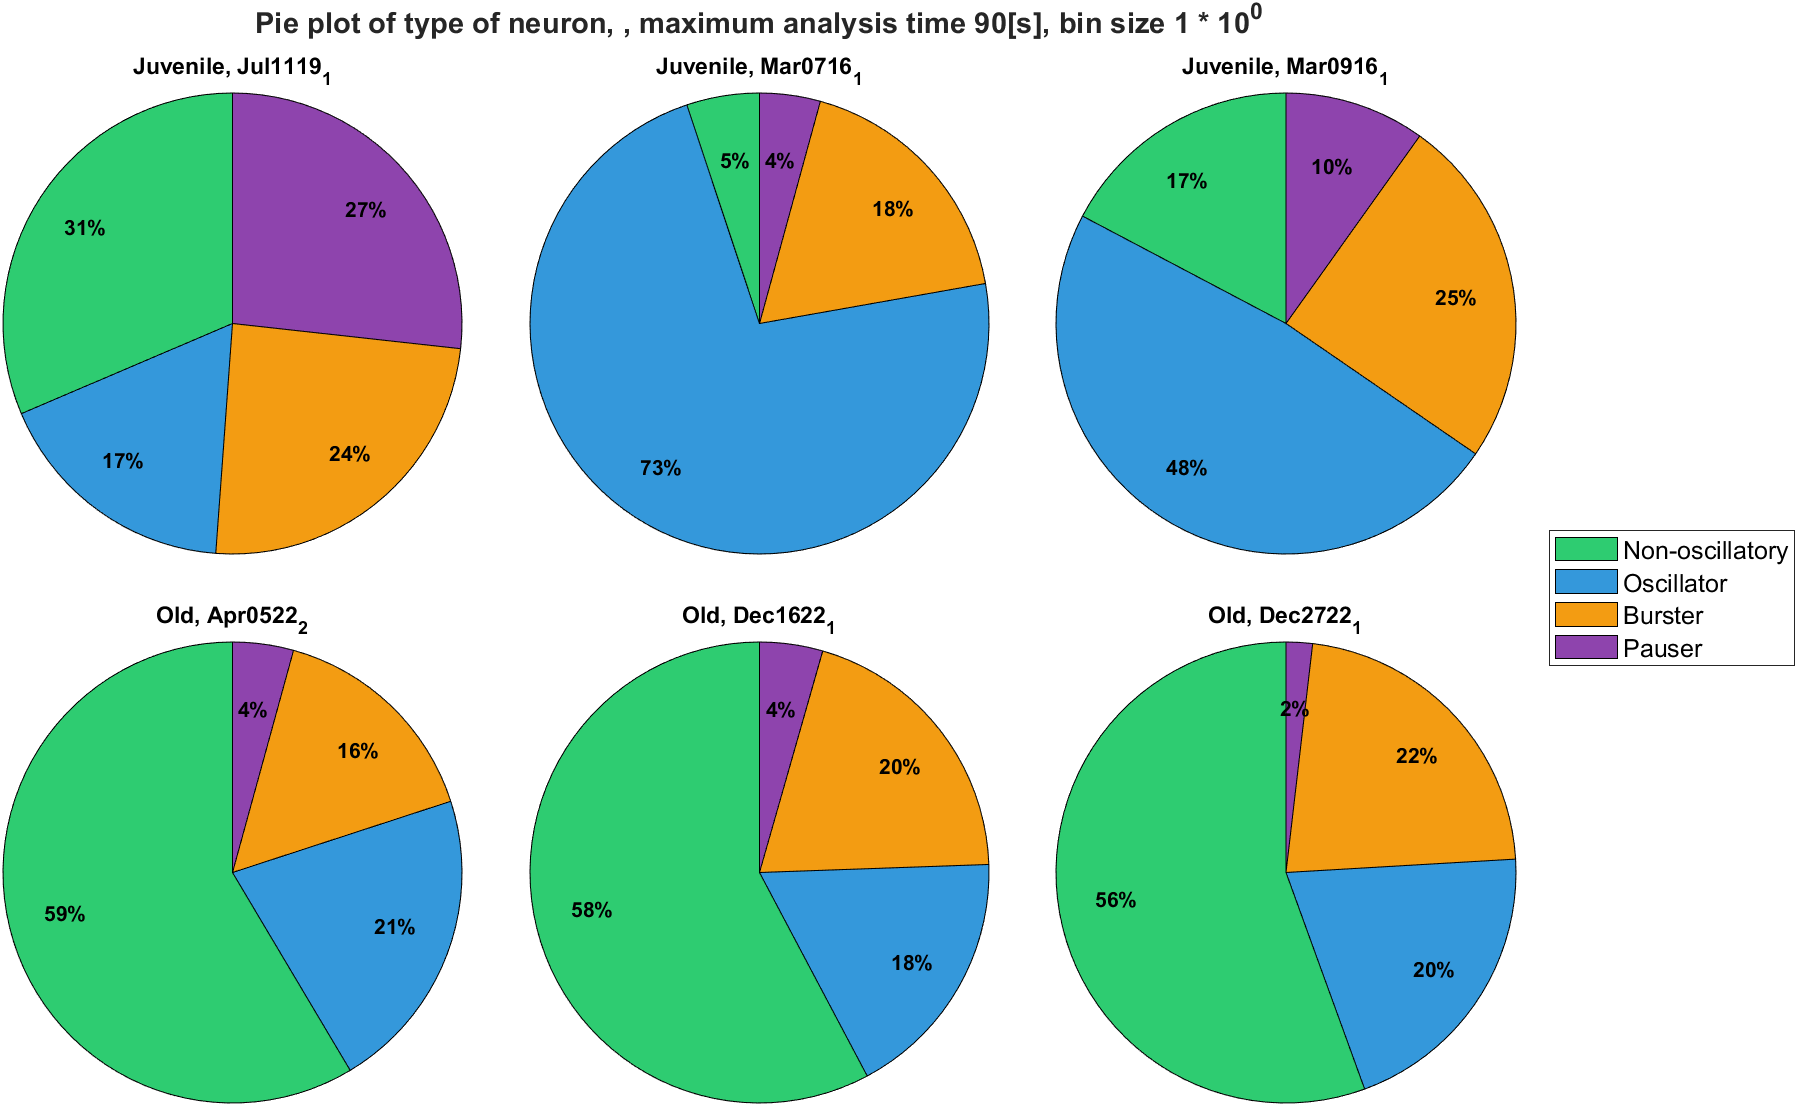
\includegraphics[width=0.7\textwidth]{img/Pie_plot_of_type_of_Neuron.png}
    \caption{Gráfico circular de total de neuronas de cada tipo por set de datos.}    
    \label{pieplot}
\end{figure}

\begin{figure}
    \centering
    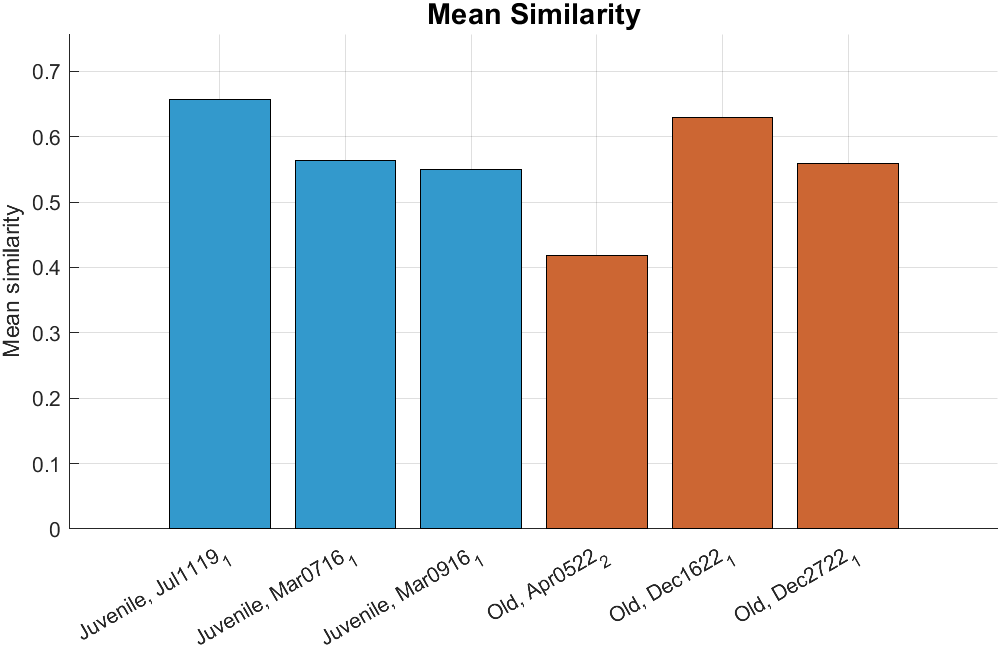
\includegraphics[width=0.7\textwidth]{img/Mean_similarity.png}
    \caption{Promedio de similaridad en matrix de similaridad del coseno por set de datos.}    
    \label{pieplot}
\end{figure}


\begin{figure}
    \centering
    \subfloat{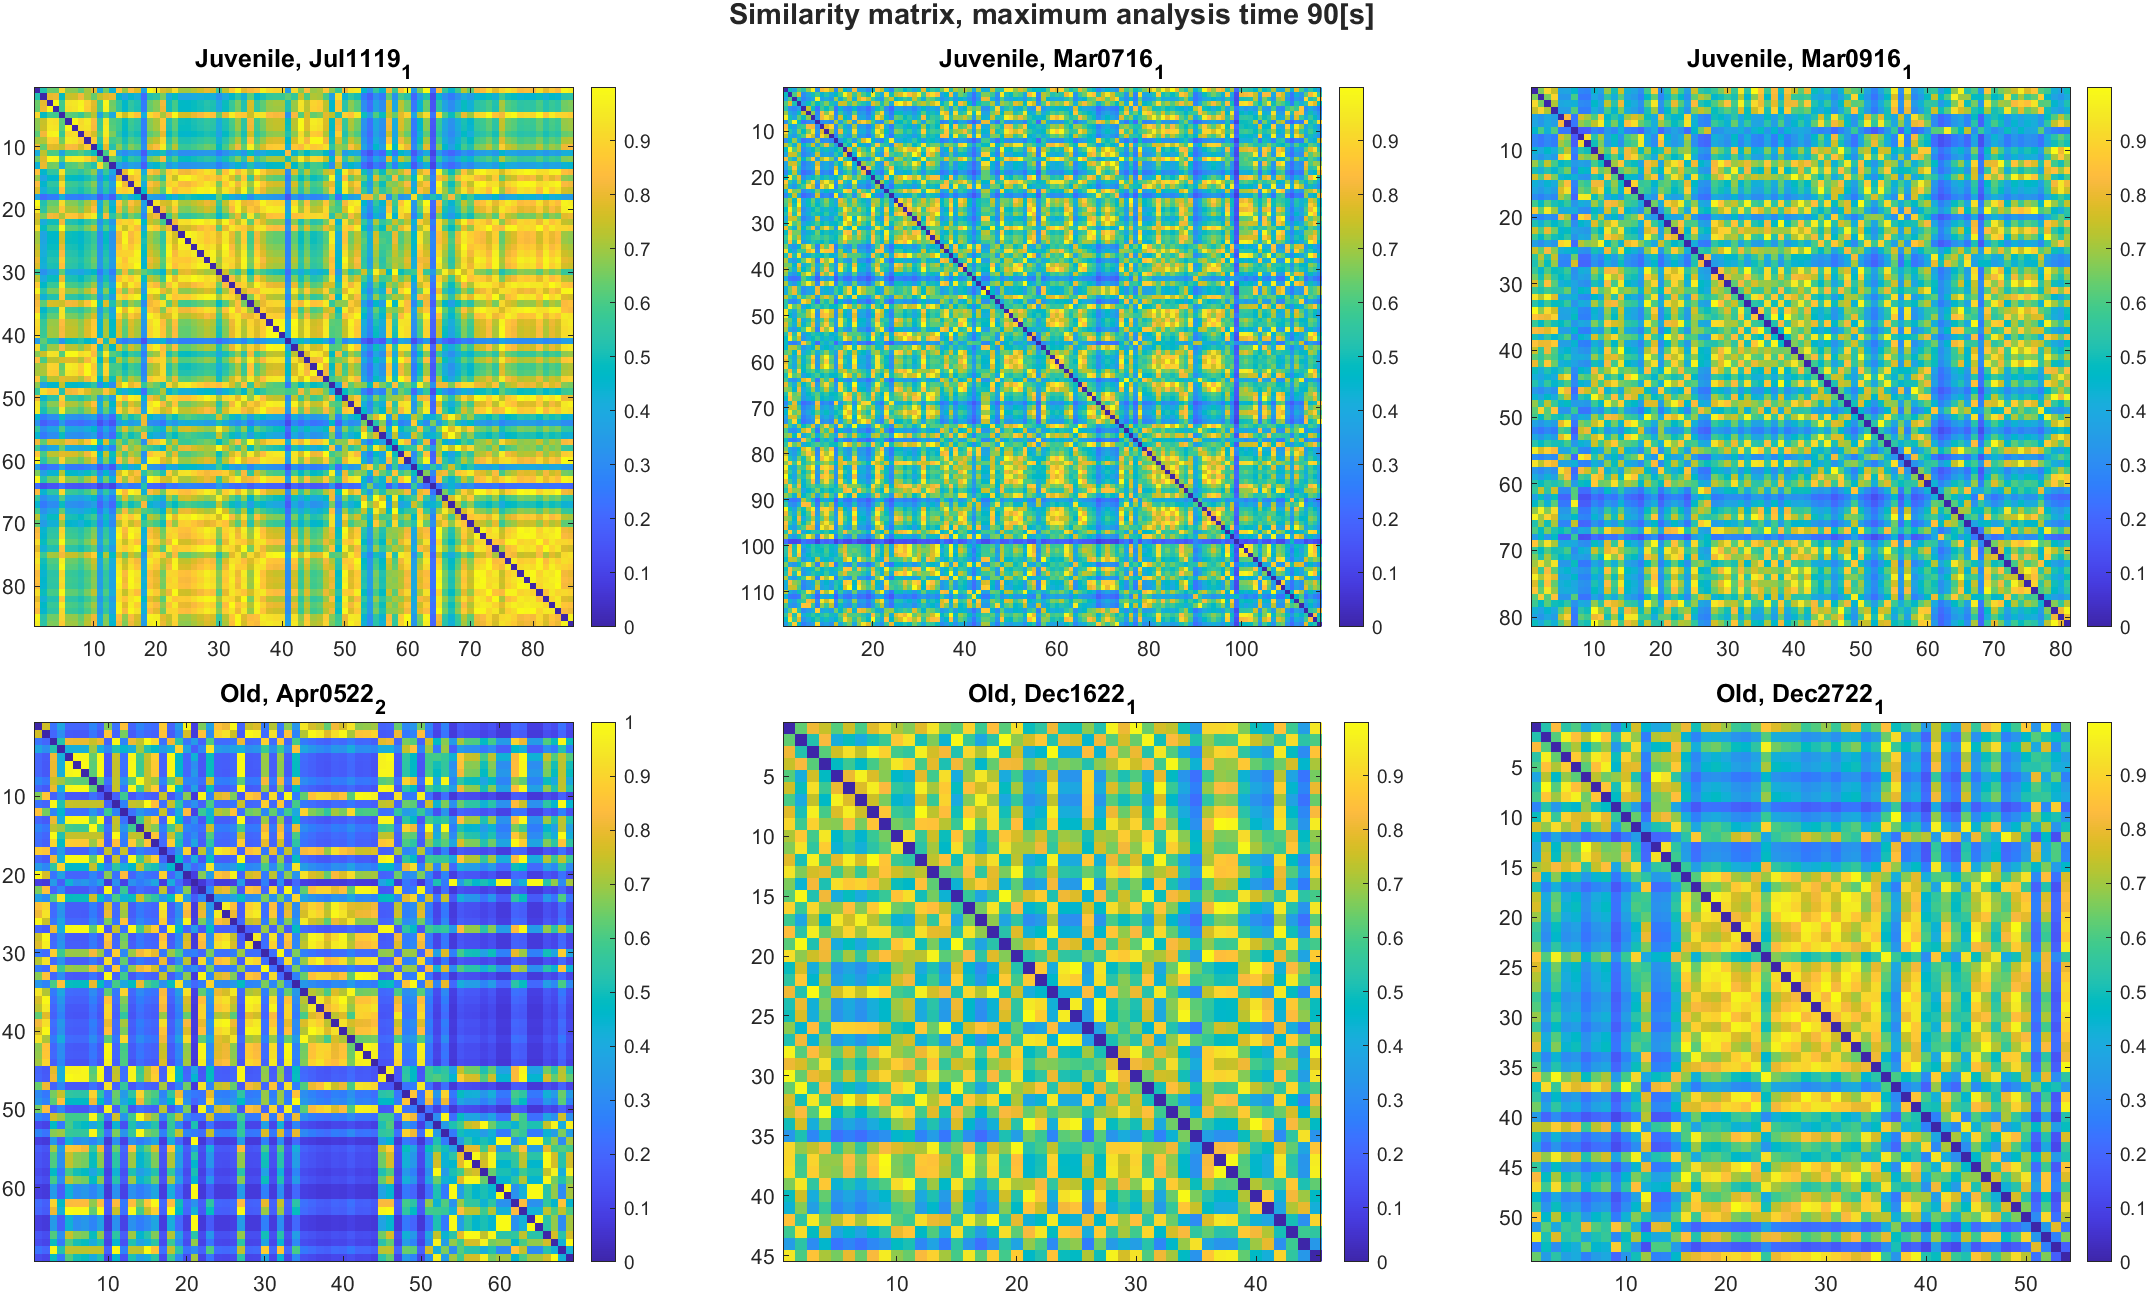
\includegraphics[width=0.9\textwidth]{img/CSM_base.png}}
    
    \hfill
    
    \subfloat{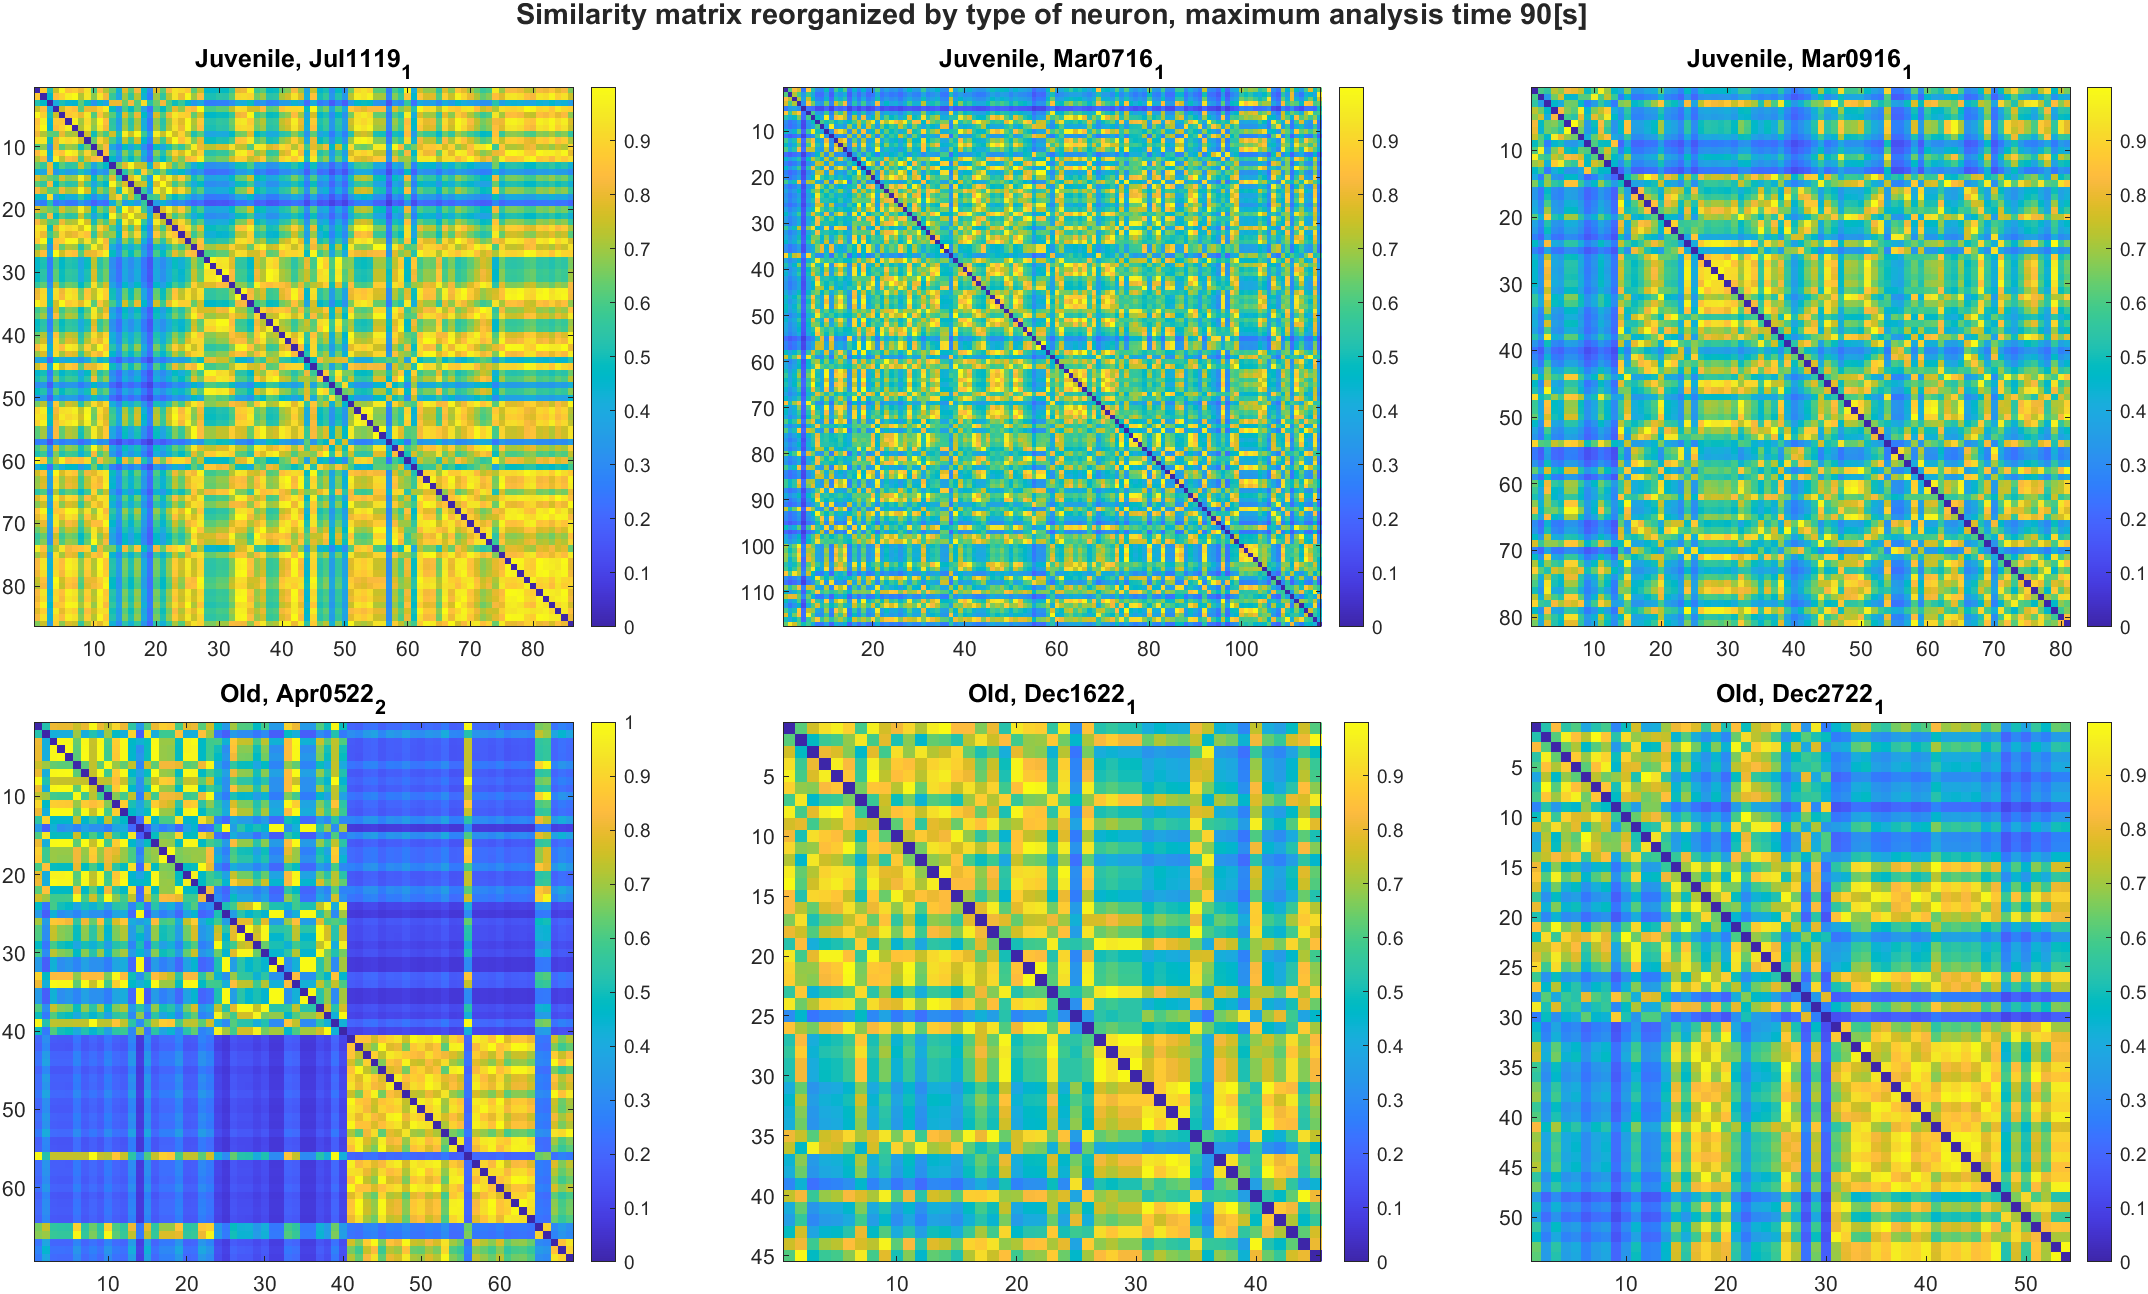
\includegraphics[width=0.9\textwidth]{img/CSM_reorganized.png}}
    
    \caption{Matriz de similaridad del coseno antes y despúes de clasificar las neuronas según patrón de disparo por set de datos.}
    
    \label{csm}
\end{figure}

\begin{figure}
    \centering
    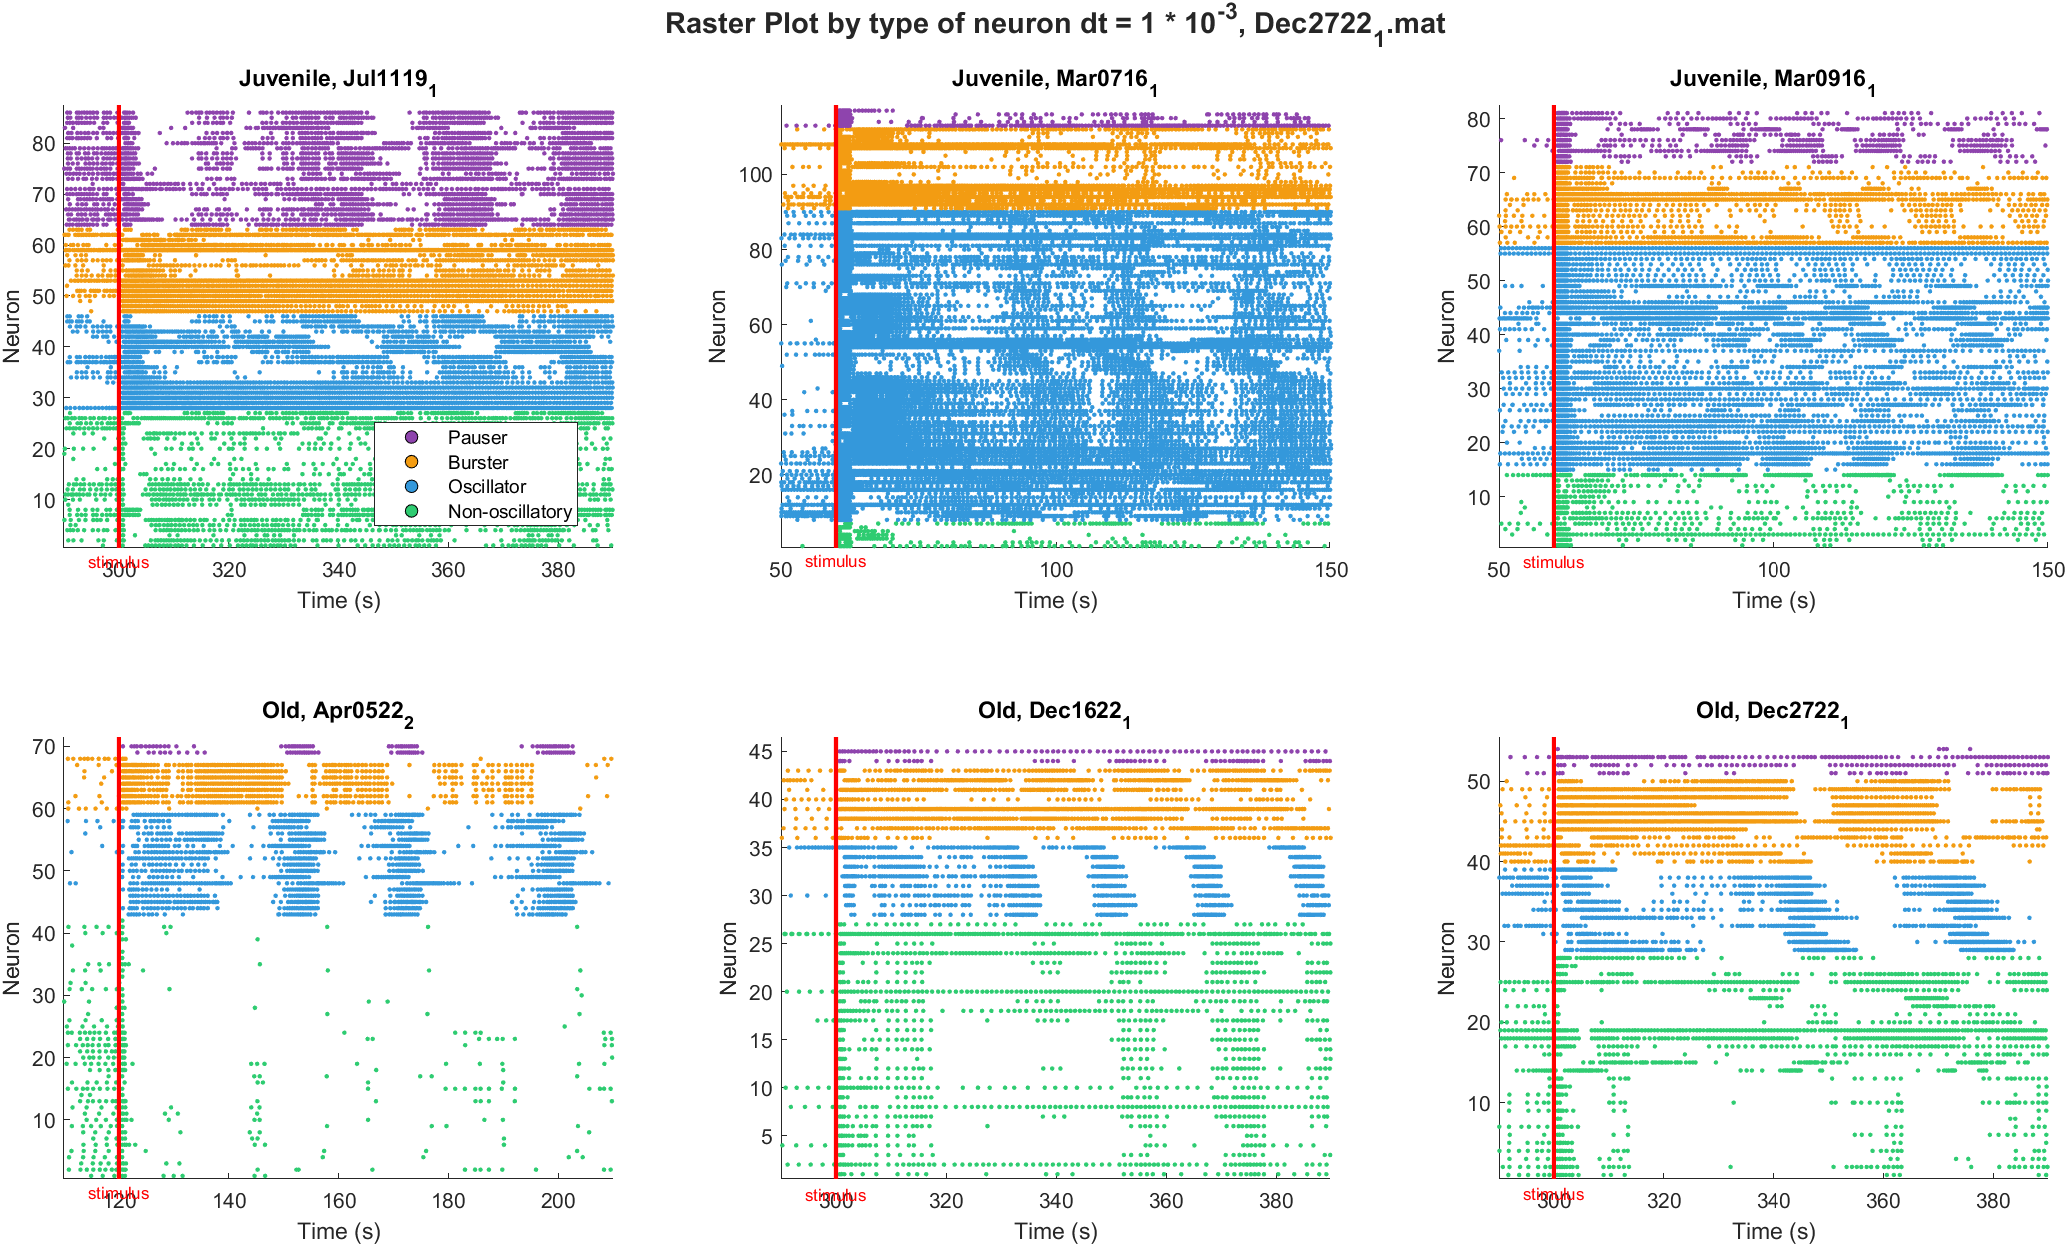
\includegraphics[width=0.9\textwidth]{img/RasterPlot_by_Type.png}
    \caption{Raster Plot con neuronas agrupadas según patrón de oscilación por set de datos.}    
    \label{RP por tipo}
\end{figure}


\begin{figure}
    \centering
    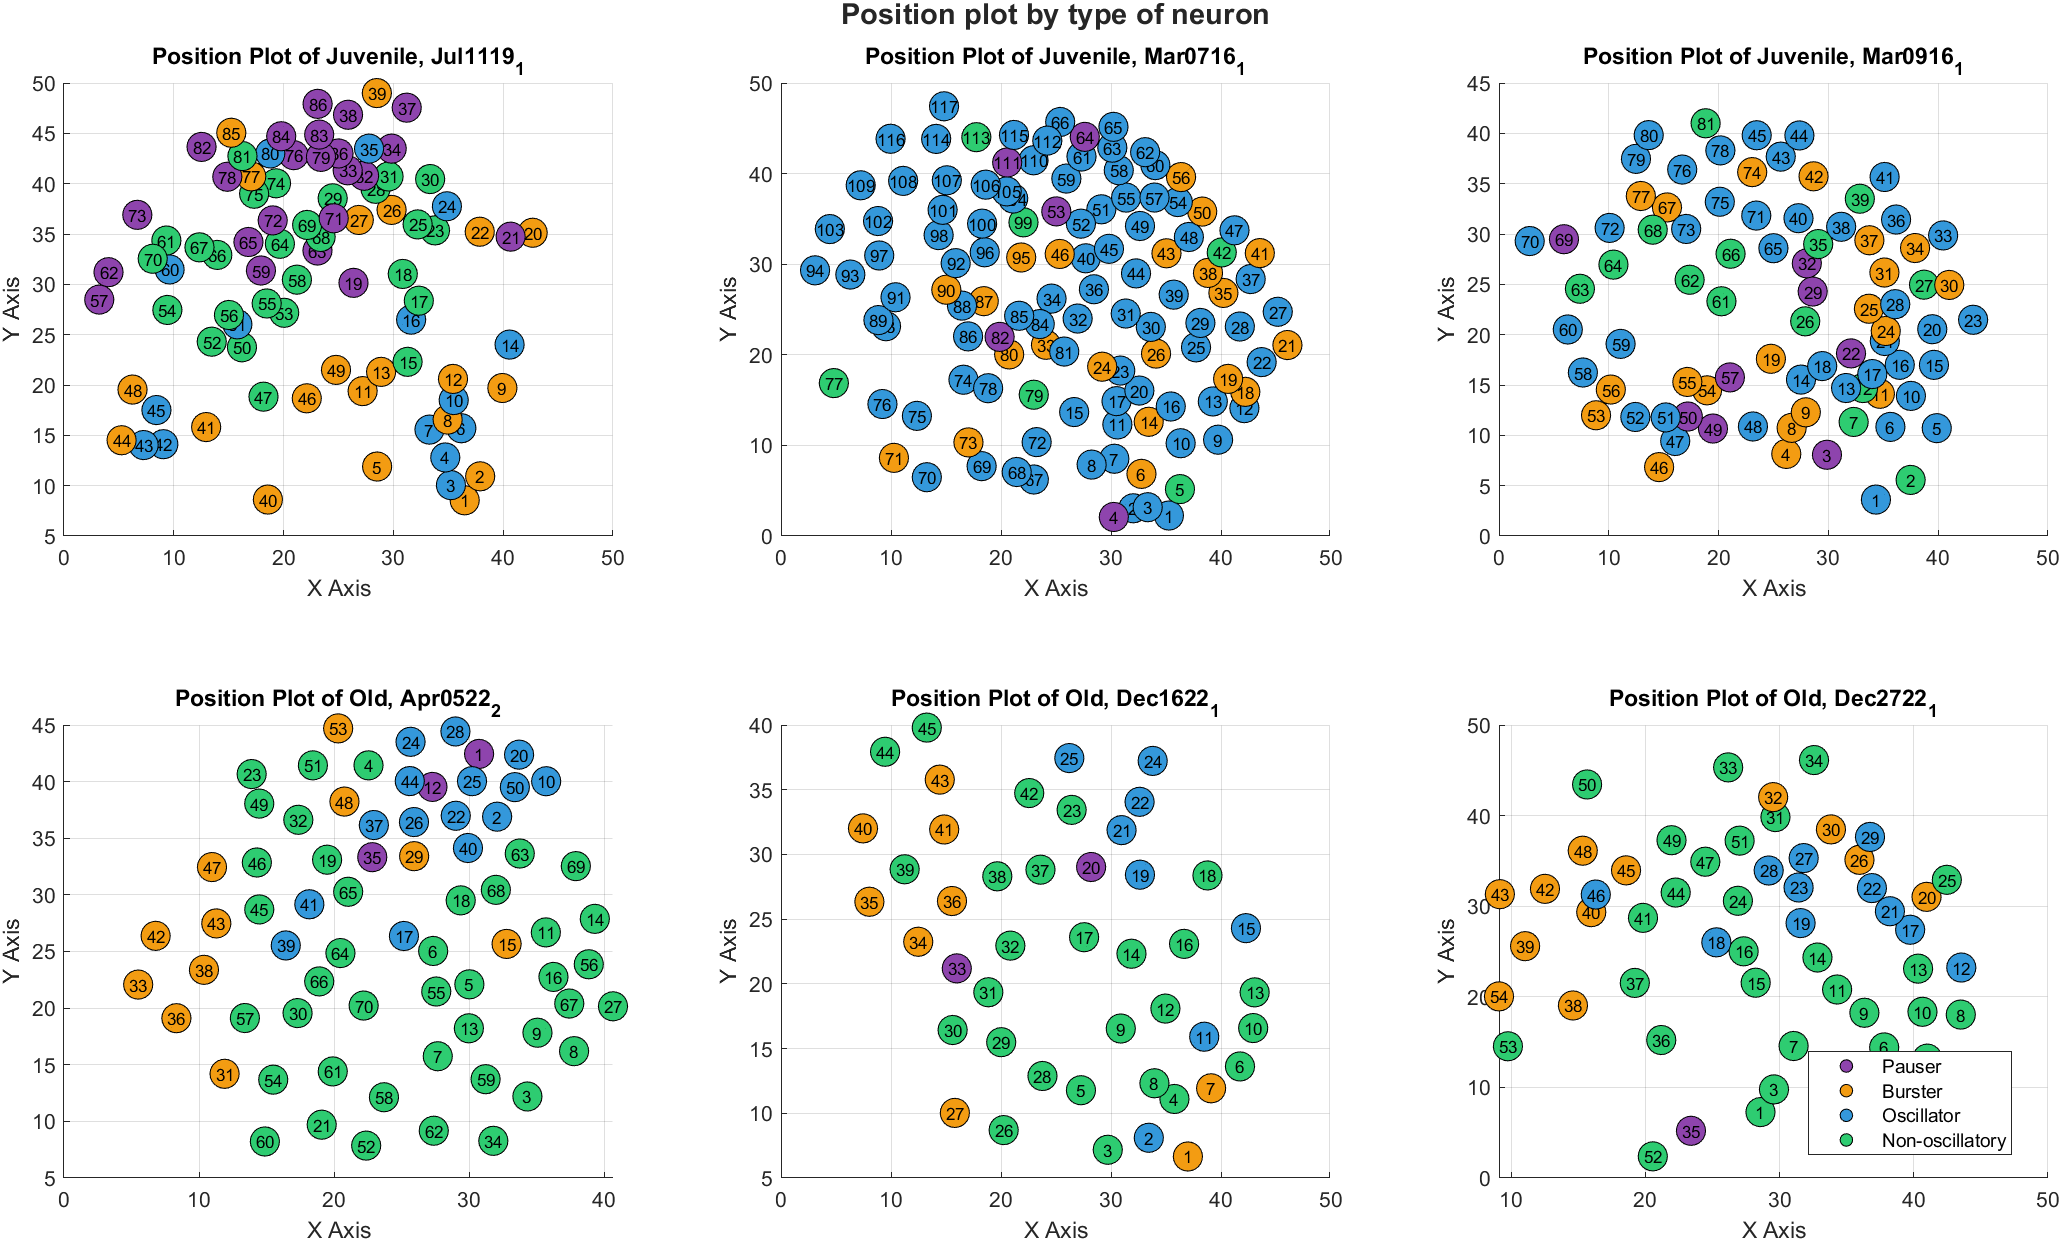
\includegraphics[width=0.9\textwidth]{img/PositionPlot_by_Type.png}
    \caption{Gráfico de posición de neuronas por dataset.}    
    \label{Positionplot}
\end{figure}

\newpage
Del trabajo realizado se concluye que, al comparar la población joven y envejecida de \textit{Aplysia}, la cantidad total de neuronas disminuye en promedio un 40\%, el promedio de spikes por tiempo, normalizado por el total de neuronas, se reduce en un 50\%, y la cantidad de neuronas oscilatorias disminuye en un 61\%. En este contexto, las neuronas no oscilatorias aumentan, mientras que las demás se mantienen en un rango similar. Finalmente, la posición relativa de los diferentes tipos de neuronas no es concluyente.\\

Se obtiene además como resultado, una carpeta de Github <\url{https://github.com/JavieraRojasM/Practica.git}> con todos los códigos de Matlab necesarios para realizar un análisis estadístico estándar de actividad neuronal y un archivo README.txt el cual contiene las instrucciones de uso de los códigos.